 \section{Aufbau und Durchführung}
\label{sec:Durchführung}

Der prinzipielle Aufbau ist bereits in Kapitel \ref{sec:phaenomene}
zu sehen. Der Aufbau zur Fokussierung des Lichts ist in Abbildung
\ref{fig:optikaufbau} zu sehen. Durch das Prisma wird das eintreffende
Licht in monochromatische Lichtstrahlen aufgeteilt. So kann garantiert
werden, dass Licht einer Wellenlänge auf die Kathode trifft.

\begin{figure}[H]
  \centering
  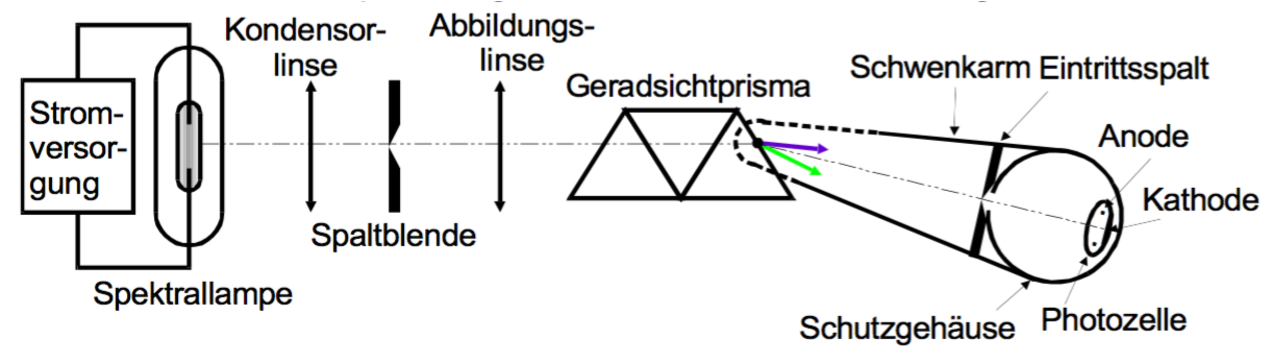
\includegraphics[width = \textwidth]{NacktbilderMilaKunis/optikaufbau.pdf}
  \caption{Optischer Teil des Versuchsaufbaus\cite{anleitung}.}
  \label{fig:optikaufbau}
\end{figure}

Der Aufbau der Photozelle ist in Abbildung \ref{fig:photozelle}
zu sehen.

\begin{figure}[H]
  \centering
  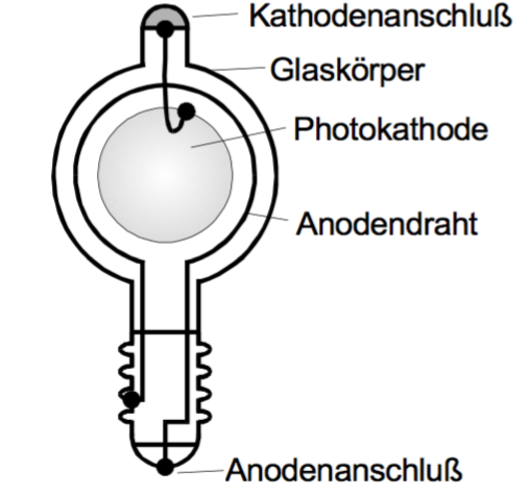
\includegraphics[height = 4cm]{NacktbilderMilaKunis/photozelle.pdf}
  \caption{Schematische Darstellung der verwendeten Photozelle\cite{anleitung}.}
  \label{fig:photozelle}
\end{figure}

Die Photozelle ist mit einer Spannungsquelle verbunden. Das Schaltbild ist in Kapitel
\ref{sec:gegenfeld} zu finden.

Nun werden zwei Messreihen durchgeführt.

\begin{itemize}
  \item Als Erstes wird für fünf verschiedene Wellenlängen die Gegenspannung $U_\g{g}$
  bestimmt bei der kein Photostrom mehr gemessen werden kann. Dann wird von da aus
  die Spannung in circa zehn Schritten auf Null verringert und der Anodenstrom vom
  Amperemeter abgelesen.
  \item Zuletzt wird die Kathode mit gelbem Licht bestrahlt und die Spannung von
  \SI{-20}{\volt} bis \SI{20}{\volt} variiert. Hierbei wird in \SI{1}{\volt}-Schritten
  vorgegangen. Nur zwischen \SI{-2}{\volt} und \SI{2}{\volt} wird genauer gemessen, nämlich
  in \SI{0.2}{\volt}-Schritten.
\end{itemize}

In den Abbildungen \ref{fig:linien}\subref{fig:linienhg} und
\ref{fig:linien}\subref{fig:linienthallium} sind die zu den Farben passende
Wellenlängen eingetragen.


\begin{figure}[H]
  \centering
  \begin{subfigure}{0.48\textwidth}
    \centering
    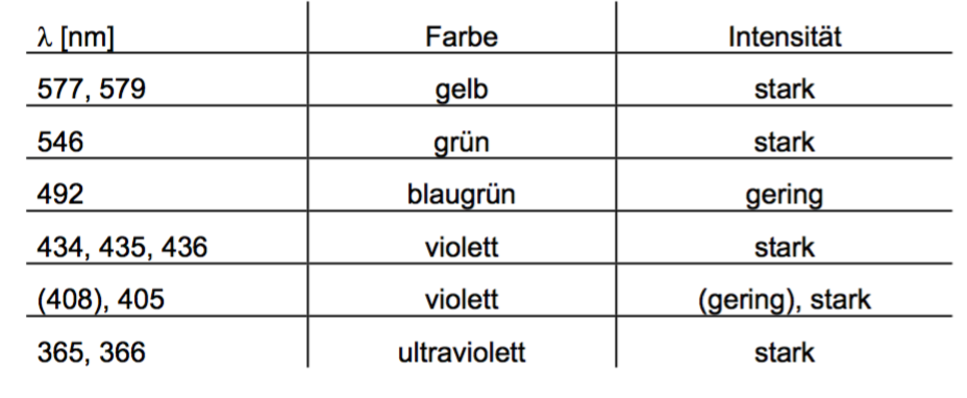
\includegraphics[width = \textwidth]{NacktbilderMilaKunis/linienhg.pdf}
    \caption{Wichtige Spektrallinien des Hg-Spektrums\cite{anleitung}.}
    \label{fig:linienhg}
  \end{subfigure}
  \begin{subfigure}{0.48\textwidth}
    \centering
    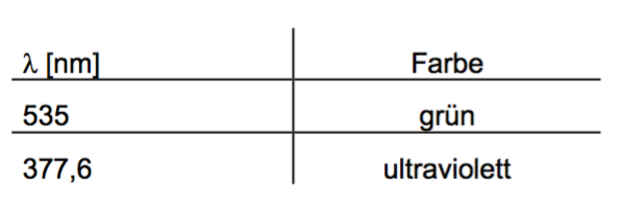
\includegraphics[width = \textwidth]{NacktbilderMilaKunis/linienthallium.pdf}
    \caption{Wichtige Linien des Thallium-Spektrums\cite{anleitung}.}
    \label{fig:linienthallium}
  \end{subfigure}
  \caption{Spektrallinien von Quecksilber und Thallium.}
  \label{fig:linien}
\end{figure}
